\documentclass{article}

\usepackage{booktabs}
\usepackage{tabularx}
\usepackage{graphicx}
\usepackage{float}

\input{../../Comments}
\input{../../Common}

\title{Usability Testing\\\progname}

\author{\authname}

\date{}

\begin{document}

\begin{table}[hp]
\caption{Revision History} \label{TblRevisionHistory}
\begin{tabularx}{\textwidth}{llX}
\toprule
\textbf{Date} & \textbf{Developer(s)} & \textbf{Change}\\
\midrule
April 2, 2025 & CG & Initial setup of document.\\
\bottomrule
\end{tabularx}
\end{table}

\newpage

\maketitle

~\newpage

\pagenumbering{roman}

\tableofcontents

\listoffigures

~\newpage

\section{Introduction}
This is the user's guide for \progname\ and is intended to provide the administrator
of the system with the necessary information to install and configure the system.
The guide will also provide both the administrator and general end users with 
information on how to use the system and its functionalities.

\section{Installation Instructions}
    \subsection{Local Installation}
        \subsubsection{Frontend Environment Configuration}
            \begin{itemize}
                \item Install Chocolatey by following the instructions:
                \href{https://docs.chocolatey.org/en-us/choco/setup/}{LINK}
                \newline The version of chocolatey used to build this project
                was 2.3.0. 
                \newline You can check your current version by running the command:
                \newline \texttt{choco --version} 
                \item Install nvm by following the instructions:
                \href{https://github.com/coreybutler/nvm-windows}{LINK}
                \newline The version of nvm used to build this project
                was 1.1.12
                \newline You can check your current version by running the command:
                \newline \texttt{nvm --version}
                \item After installing nvm, you will need to install nodejs.
                \newline You can do this by running the following commands (in order):
                \newline \texttt{nvm install 20.18.0}
                \newline \texttt{nvm use 20.18.0}
                \newline You can check your current version by running the command:
                \newline \texttt{nvm current}
                \item The npm version used to build this project was 10.8.2
                \newline You can check your current version by running the command:
                \newline \texttt{npm --version}
                \item Locally install the nodejs packages listed in the repository's 
                package.json file by running the command:
                \newline \texttt{npm install}
                \newline within the \texttt{src/website/sandlot} directory of the 
                repository.
                \item Create a .env file in the \texttt{src/website/sandlot} directory
                of the repository and copy the contents below into it:
                \newline \texttt{REACT\_APP\_API\_URL=http://localhost:8000}
            \end{itemize}
        \subsubsection{Backend Environment Configuration}
            \begin{itemize}
                \item Install Python by following the instructions:
                \href{https://www.python.org/downloads/}{LINK}
                \newline The version of python used to build this project
                was 3.13.0
                \newline You can check your current version by running the command:
                \newline \texttt{python --version}
                \item The pip version used to build this project was 24.3.1
                \newline You can check your current version by running the command:
                \newline \texttt{pip --version}
                \item Install pipenv by running the command:
                \newline \texttt{pip install pipenv}
                \newline The versdion of pipenv used to build this project was 2024.4.0
                \newline You can check your current version by running the command:
                \newline \texttt{pipenv --version}
                \item Locally install the python packages listed in the repository's 
                Pipfile file by running the command:
                \newline \texttt{pipenv install}
                \newline within the \texttt{src/backend} directory of the 
                repository.
                \item Create a .env file in the \texttt{src/backend} directory
                of the repository and copy the contents below into it:
                \newline \texttt{CONN\_STRING=your-connection-string-here}
                \newline \texttt{REMOTE\_HOST=http://localhost:3000}
            \end{itemize}
        \subsubsection{Running the Application}
            \begin{itemize}
                \item To run the backend, open a terminal and run the command:
                \newline \texttt{fastapi dev main.py}
                \newline within the \texttt{src/backend/app} directory of the 
                repository.
                \item To run the frontend, open a second terminal and run the command:
                \newline \texttt{npm run dev}
                \newline within the \texttt{src/website/sandlot} directory of the 
                repository.
            \end{itemize}
        \subsubsection{Potential Issues}
            \begin{itemize}
                \item If you are having issues with installations try closing and re-opening
                your terminal/IDE
                \item You may need install Visual Studio Community 2022 from: 
                \href{https://visualstudio.microsoft.com/vs/community/}{LINK}
                \item If you're getting the error message:
                \newline \texttt{node-gyp error Could not find any Visual Studio installation to use}
                \newline Use the following link to troubleshoot the issue:
                \href{https://stackoverflow.com/questions/70315519/node-gyp-error-could-not-find-any-visual-studio-installation-to-use}{LINK}
            \end{itemize}

\section{Features}
    \subsection{Commissioner}
            \subsubsection{Announcements}
                When logged in as a commissioner, announcements visible to
                all users can be created, edited, and deleted from the home page.
                \newline 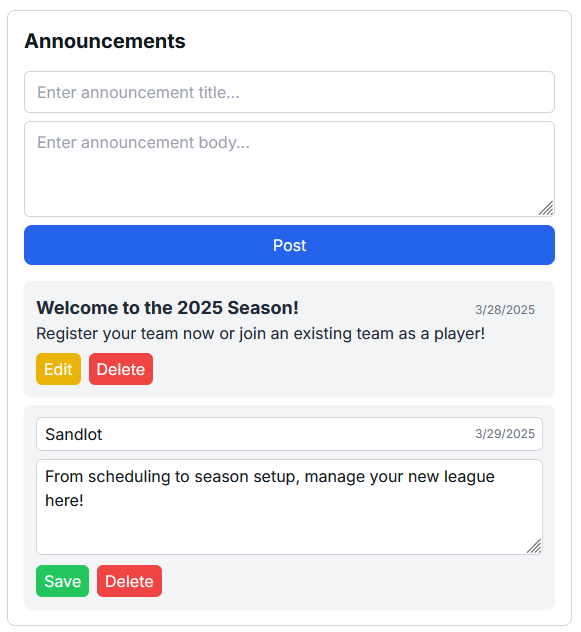
\includegraphics[scale=0.6]{announcements.png}
            \subsubsection{Team Directory}
                When logged in as a commissioner, the team directory can be accessed
                from the home page. Additionally, selecting reveals a dropdown which
                displays all members of the team, their information, and a copy
                of their signed waiver available for download.
                \newline 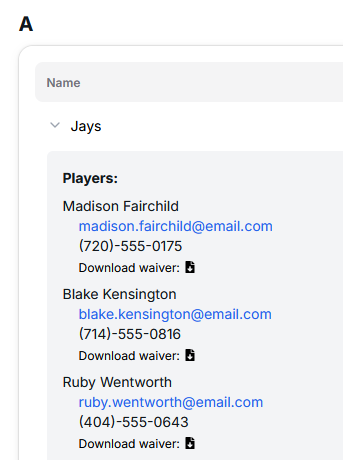
\includegraphics[scale=0.6]{team-directory.png}
            \subsubsection{Waiver Page}
                When logged in as a commissioner, the waiver page can be accessed
                from the navigation bar in the manage league dropdown. The waiver page 
                allows the commissioner to determine whether players are required to sign
                a waiver on registration via the "Enable Waiver" switch at the top of the 
                page. The waiver page also allows the commissioner to customize the waiver
                text and title that users must sign on registration by creating, editing, and
                deleting waiver fields. Any changes made to the waiver page will be saved only 
                if the "Save Configuration" button is clicked before navigating away from the 
                page.
                \newline 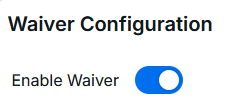
\includegraphics[scale=0.6]{enable-waiver.png}
                \newline 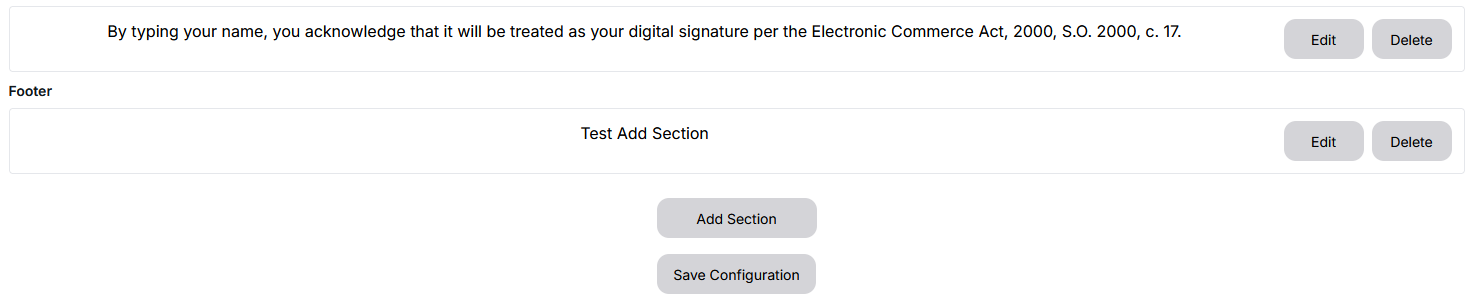
\includegraphics[scale=0.4]{waiver-management.png}
                \newline 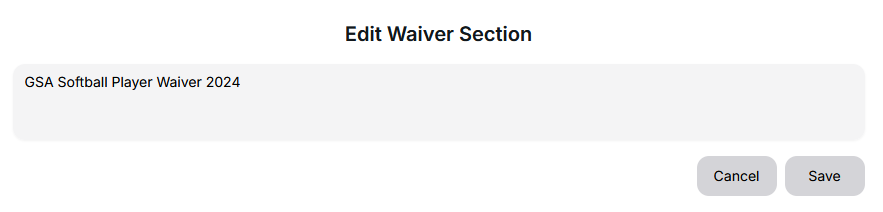
\includegraphics[scale=0.6]{edit-waiver.png}
            \subsubsection{}
    \subsection{Team}
    \subsection{Player}
    \subsection{All Users}

\end{document}